\documentclass[12pt,a4paper]{article}
\usepackage[polish]{babel}
\usepackage[T1]{fontenc}
\usepackage[utf8]{inputenc}
% \usepackage{hyperref}
\usepackage{url}
\usepackage{graphicx}

\addtolength{\hoffset}{-1.5cm}
\addtolength{\marginparwidth}{-1.5cm}
\addtolength{\textwidth}{3cm}
\addtolength{\voffset}{-1cm}
\addtolength{\textheight}{2.5cm}
\setlength{\topmargin}{0cm}
\setlength{\headheight}{0cm}

\usepackage{listings}
\usepackage{xcolor}

\definecolor{codegreen}{rgb}{0,0.6,0}
\definecolor{codegray}{rgb}{0.5,0.5,0.5}
\definecolor{codepurple}{rgb}{0.58,0,0.82}
\definecolor{backcolour}{rgb}{0.95,0.95,0.92}

\lstdefinelanguage{JavaScript}{
  keywords={typeof, new, true, false, catch, function, return, null, catch, switch, var, if, in, while, do, else, case, break},
  keywordstyle=\color{blue}\bfseries,
  ndkeywords={class, export, boolean, throw, implements, import, this},
  ndkeywordstyle=\color{darkgray}\bfseries,
  identifierstyle=\color{black},
  sensitive=false,
  comment=[l]{//},
  morecomment=[s]{/*}{*/},
  commentstyle=\color{codegreen}\ttfamily,
  stringstyle=\color{codepurple}\ttfamily,
  morestring=[b]',
  morestring=[b]"
}

\lstdefinestyle{mystyle}{
  language=JavaScript,
  backgroundcolor=\color{backcolour},
  commentstyle=\color{codegreen},
  keywordstyle=\color{magenta},
  numberstyle=\tiny\color{codegray},
  stringstyle=\color{codepurple},
  basicstyle=\ttfamily\footnotesize,
  breakatwhitespace=false,
  breaklines=true,
  captionpos=b,
  keepspaces=true,
  numbers=left,
  numbersep=5pt,
  showspaces=false,
  showstringspaces=false,
  showtabs=false,
  tabsize=2
}

\lstset{style=mystyle}


\begin{document}


\title{Dokumentacja projektowa Kryptografia i teoria kodów}
\author{Nikodem Bulanda}
\date{\today}

\maketitle


Autor:
\begin{itemize}
\item[] Bartłomiej Cetera
\end{itemize}


\newpage

\tableofcontents


\newpage
\section{Wstęp}

\subsection{Czym jest kryptografia?}
\noindent Kryptografia to dziedzina nauki zajmująca się technikami szyfrowania informacji w celu zapewnienia ich poufności, integralności, autentyczności i niezaprzeczalności. W praktyce oznacza to metody zmieniania czytelnej wiadomości (tekst jawny) na formę trudną do odczytania (szyfrogram) oraz możliwość przywrócenia jej do pierwotnej postaci. Kryptografia znajduje zastosowanie w zabezpieczaniu komunikacji, danych w sieci, uwierzytelnianiu użytkowników oraz wielu innych dziedzinach, takich jak podpisy cyfrowe czy blockchain.\newline

\textbf{Podstawowe pojęcia w kryptografii:}
\begin{itemize}
\item Szyfrowanie: Proces zmiany tekstu jawnego w szyfrogram za pomocą algorytmu i klucza.
\item Klucz: Sekretny parametr używany w procesach szyfrowania i deszyfrowania.
\item Kryptografia symetryczna: Wykorzystuje ten sam klucz do szyfrowania i deszyfrowania.
\item Kryptografia asymetryczn: Wykorzystuje parę kluczy – publiczny do szyfrowania i prywatny do deszyfrowania.
\end{itemize}

\subsection{Algorytmy}
\subsubsection{AES}
\noindent\textbf{Opis}
\begin{quotation}\noindent AES (Advanced Encryption Standard) to algorytm szyfrowania symetrycznego, który został przyjęty jako standard szyfrowania przez Narodowy Instytut Standaryzacji i Technologii (NIST) w 2001 roku. Został opracowany przez belgijskich kryptografów Vincenta Rijmena i Joana Daemena i początkowo nazwany Rijndael. AES zastąpił starszy standard DES (Data Encryption Standard) ze względu na wyższy poziom bezpieczeństwa i lepszą wydajność.\end{quotation}

\noindent\textbf{Zasada działania}
\begin{quotation}\noindent AES to szyfr blokowy, co oznacza, że dane są dzielone na bloki o stałym rozmiarze (128 bitów) i szyfrowane w każdym bloku niezależnie. Algorytm wykonuje szereg operacji matematycznych na danych w kilku rundach (10, 12 lub 14, w zależności od długości klucza: 128, 192 lub 256 bitów). Proces szyfrowania składa się z następujących etapów:
\begin{itemize}
\item SubBytes: Zastępowanie bajtów według tabeli S-box (substytucja).
\item ShiftRows: Przesunięcie wierszy macierzy w lewo.
\item MixColumns: Operacja mieszania kolumn w celu większego rozproszenia danych.
\item AddRoundKey: Łączenie danych z kluczem szyfrowania za pomocą operacji XOR.
\end{itemize}
\end{quotation}

\noindent\textbf{Zastosowanie}
\begin{quotation}\noindent AES jest popularny dzięki swojej efektywności, bezpieczeństwu i wsparciu na wielu platformach sprzętowych i programowych. Jest odporny na większość znanych ataków kryptograficznych i spełnia wymagania związane z ochroną danych na wysokim poziomie. AES jest powszechnie używany do ochrony danych w różnych dziedzinach:
\begin{itemize}
\item Szyfrowanie komunikacji: Protokół HTTPS, VPN, komunikatory.
\item Ochrona plików: Szyfrowanie dysków twardych i plików.
\item Bankowość i finanse: Bezpieczeństwo transakcji online.
\item Urządzenia mobilne: Szyfrowanie danych w telefonach i aplikacjach.
\item Rząd i wojsko: Ochrona danych niejawnych i wrażliwych.
\end{itemize}
\end{quotation}


\subsubsection{DES}
\noindent\textbf{Opis}
\begin{quotation}\noindent DES (Data Encryption Standard) to algorytm szyfrowania symetrycznego, który został opracowany w latach 70. XX wieku przez IBM i zatwierdzony jako standard szyfrowania przez Narodowy Instytut Standaryzacji i Technologii (NIST) w 1977 roku. Był to jeden z pierwszych szeroko stosowanych algorytmów kryptograficznych w komputerach. DES opiera się na pracy Horsta Feistela i jego strukturze kryptograficznej. Ze względu na zbyt małą długość klucza (56 bitów), DES stał się podatny na ataki brute force i został zastąpiony przez AES w 2001 roku.
\end{quotation}

\noindent\textbf{Zasada działania}
\begin{quotation}\noindent DES to szyfr blokowy, który operuje na blokach danych o stałym rozmiarze 64 bitów i wykorzystuje klucz o długości 56 bitów. Algorytm wykonuje 16 rund szyfrowania, w każdej z nich stosując różne operacje kryptograficzne:
\begin{itemize}
\item Permutacja początkowa (IP): Dane wejściowe są przeorganizowane w określony sposób.
\item Podział na półbloki: Blok danych jest dzielony na dwie części (lewa i prawa).
\item Feistel function: W każdej rundzie prawa część jest przetwarzana z użyciem klucza i funkcji kryptograficznej, a następnie łączona z lewą częścią przy pomocy operacji XOR.
\item Permutacja końcowa (FP): Po 16 rundach dane są ponownie permutowane.
\end{itemize}
\end{quotation}

\noindent\textbf{Zastosowanie}
\begin{quotation}\noindent DES w swoich czasach był uznawany za bezpieczny i wydajny, dzięki czemu zyskał dużą popularność. Był jednym z pierwszych algorytmów szyfrowania zaimplementowanych na szeroką skalę i zapoczątkował rozwój nowoczesnej kryptografii. Jednak z czasem długość klucza okazała się zbyt krótka, a algorytm został uznany za przestarzały i podatny na ataki brute force. Obecnie DES jest głównie używany w celach edukacyjnych lub w formie ulepszonej jako Triple DES (3DES), który zwiększa długość klucza i odporność na ataki. DES był szeroko stosowany w latach 80. i 90. XX wieku w następujących obszarach:
\begin{itemize}
\item Bankowość: Szyfrowanie transakcji bankomatowych (ATM) i kart kredytowych.
\item Sieci telekomunikacyjne: Ochrona komunikacji głosowej i tekstowej.
\item Przemysł: Ochrona danych w systemach informatycznych firm.
\item Rząd: Bezpieczeństwo danych niejawnych (do lat 90.).
\end{itemize}
\end{quotation}



\subsubsection{RSA}
\noindent\textbf{Opis}
\begin{quotation}\noindent RSA (od nazwisk wynalazców: Ron Rivest, Adi Shamir i Leonard Adleman) to jeden z pierwszych publicznych algorytmów kryptograficznych, który opiera się na asymetrycznym szyfrowaniu. Algorytm został zaprezentowany w 1977 roku na MIT i szybko stał się podstawowym narzędziem w dziedzinie kryptografii. RSA jest oparty na teorii liczb i trudności faktoryzacji dużych liczb pierwszych.
\end{quotation}

\noindent\textbf{Zasada działania}
\begin{quotation}\noindent RSA to algorytm kryptograficzny asymetryczny, który wykorzystuje parę kluczy: klucz publiczny i klucz prywatny. Jego działanie opiera się na trudności faktoryzacji dużych liczb pierwszych.

\noindent\textbf{Generowanie kluczy}
\begin{itemize}
    \item Wybierz dwie duże liczby pierwsze \( p \) i \( q \).
    \item Oblicz moduł \( n \) jako iloczyn \( p \) i \( q \):
    \[
    n = p \times q
    \]
    \item Oblicz funkcję Eulera \( \phi(n) \):
    \[
    \phi(n) = (p - 1) \times (q - 1)
    \]
    \item Wybierz liczbę \( e \), która spełnia warunek \( 1 < e < \phi(n) \) oraz jest względnie pierwsza z \( \phi(n) \).
    \item Oblicz klucz prywatny \( d \) jako odwrotność modularną \( e \) względem \( \phi(n) \):
    \[
    d \cdot e \equiv 1 \ (\text{mod} \ \phi(n))
    \]
\end{itemize}

\noindent\textbf{Szyfrowanie}
Wiadomość \( m \) jest szyfrowana za pomocą klucza publicznego \( (e, n) \) zgodnie z równaniem:
\[
c = m^e \ \text{mod} \ n
\]
gdzie \( c \) to szyfrogram.

\subsection*{Deszyfrowanie}
Szyfrogram \( c \) jest odszyfrowywany za pomocą klucza prywatnego \( (d, n) \) zgodnie z równaniem:
\[
m = c^d \ \text{mod} \ n
\]
gdzie \( m \) to odszyfrowana wiadomość.

\end{quotation}

\noindent\textbf{Zastosowanie}
\begin{quotation}\noindent RSA zrewolucjonizował kryptografię, ponieważ umożliwił szyfrowanie asymetryczne, eliminując konieczność uprzedniego wymieniania klucza prywatnego między stronami. Algorytm opiera się na solidnym matematycznym fundamencie (trudności faktoryzacji dużych liczb pierwszych), co czyni go bardzo bezpiecznym. Jest jednak stosunkowo wolny w porównaniu z algorytmami symetrycznymi, dlatego często używa się go w połączeniu z szyfrowaniem symetrycznym, np. w systemach hybrydowych (RSA + AES). RSA jest powszechnie stosowany w:
\begin{itemize}
\item Protokołach bezpieczeństwa internetowego (SSL/TLS): Służy do ustanawiania bezpiecznych połączeń w internecie.
\item Szyfrowaniu poczty elektronicznej: Programy takie jak PGP wykorzystują RSA do szyfrowania i podpisywania wiadomości.
\item Podpisach cyfrowych: Zapewnia autentyczność i integralność danych.
\item Dystrybucji kluczy: RSA jest używany do bezpiecznego przekazywania kluczy w algorytmach symetrycznych.
\end{itemize}
\end{quotation}



\subsubsection{Szyfr Monoalfabetyczny}
\noindent\textbf{Opis}
\begin{quotation}\noindent Szyfr monoalfabetyczny, znany również jako szyfr podstawieniowy, jest jednym z najstarszych i najprostszych algorytmów szyfrowania. Szyfr monoalfabetyczny był szeroko stosowany w starożytności, zwłaszcza w czasach rzymskich. Julius Caesar używał uproszczonej wersji tego szyfru, znanej jako szyfr Cezara, aby zabezpieczać swoje wiadomości wojskowe. Pomimo prostoty, przez wieki był podstawowym narzędziem w kryptografii, zanim pojawiły się bardziej zaawansowane metody.
\end{quotation}

\noindent\textbf{Zasada działania}
\begin{quotation}\noindent Szyfr monoalfabetyczny działa na zasadzie podstawienia każdej litery tekstu jawnego na inną literę zgodnie z ustalonym kluczem, który definiuje mapowanie znaków. Klucz to permutacja alfabetu, gdzie każdej literze alfabetu jawnego odpowiada inna litera alfabetu szyfrowego.\newline

\noindent\textbf{Proces szyfrowania:}
\begin{itemize}
\item Każda litera tekstu jawnego jest zastępowana odpowiednią literą z klucza szyfrowania.
\item Spacje, cyfry i znaki interpunkcyjne mogą być pozostawione bez zmian lub również szyfrowane, w zależności od implementacji.
\end{itemize}

\noindent\textbf{Proces deszyfrowania:}
\begin{itemize}
\item Każda litera szyfrogramu jest zastępowana literą tekstu jawnego zgodnie z odwrotną permutacją klucza.
\end{itemize}
\end{quotation}

\noindent\textbf{Zastosowanie}
\begin{quotation}\noindent Szyfr monoalfabetyczny był stosowany w korespondencji wojskowej i dyplomatycznej, aby ukryć znaczenie wiadomości.Dzisiaj szyfr monoalfabetyczny ma znaczenie głównie edukacyjne, jako wprowadzenie do kryptografii. Ze względu na łatwość złamania przy użyciu analizy częstotliwości, nie jest już używany w praktycznych zastosowaniach bezpieczeństwa.
\end{quotation}



\subsubsection{Szyfr Transpozycyjny}
\noindent\textbf{Opis}
\begin{quotation}\noindent Szyfr transpozycyjny to technika kryptograficzna, w której znaki tekstu jawnego są przemieszczane (transponowane) zgodnie z określonym wzorcem lub regułą, zamiast być zastępowane innymi znakami. Szyfry transpozycyjne były używane już w starożytności. Jednym z najwcześniejszych przykładów jest skytale, narzędzie stosowane przez starożytnych Spartan do szyfrowania wiadomości. Wiadomość była zapisywana na pasku pergaminu owiniętym wokół cylindrycznego obiektu, a jej odczytanie wymagało odpowiedniego klucza w postaci cylindra o tej samej średnicy.
\end{quotation}

\noindent\textbf{Zasada działania}
\begin{quotation}\noindent Szyfr transpozycyjny zmienia kolejność liter w tekście jawnym według określonego klucza, ale nie zmienia samych znaków.\newline

\noindent\textbf{Proces szyfrowania:}
\begin{itemize}
\item Tekst jawny jest wpisywany w siatkę lub według ustalonego wzorca.
\item Znaki są odczytywane w innej kolejności, zgodnie z kluczem.
\item Wynik to szyfrogram, który zawiera te same znaki co tekst jawny, ale w zmienionej kolejności.
\end{itemize}

\noindent\textbf{Proces deszyfrowania:}
\begin{itemize}
\item Szyfrogram jest wpisywany w siatkę zgodnie z kluczem.
\item Odczytuje się znaki w pierwotnej kolejności, aby odzyskać tekst jawny.
\end{itemize}
\end{quotation}

\noindent\textbf{Zastosowanie}
\begin{quotation}\noindent  Szyfry transpozycyjne były wykorzystywane w czasach wojny do ukrywania wiadomości, zwłaszcza tam, gdzie urządzenia do bardziej zaawansowanego szyfrowania nie były dostępne. Szyfr transpozycyjny ma głównie zastosowanie edukacyjne i teoretyczne w nauce kryptografii, aby pokazać różnicę między szyframi podstawieniowymi a transpozycyjnymi.
\end{quotation}


\subsubsection{HMAC}
\noindent\textbf{Opis}
\begin{quotation}\noindent HMAC (Hashed Message Authentication Code) to mechanizm kryptograficzny służący do uwierzytelniania wiadomości oraz zapewnienia ich integralności przy użyciu funkcji skrótu i klucza tajnego. HMAC został formalnie opisany w 1996 roku przez Mihira Bellare, Ranju Canettiego i Hugo Krawczyka. Jest szeroko stosowany w kryptografii, w szczególności w protokołach uwierzytelniania i komunikacji, takich jak TLS, IPsec czy JWT. HMAC został zaprojektowany jako bezpieczny i łatwy w implementacji sposób na wykorzystanie funkcji skrótu w celu uwierzytelniania danych.
\end{quotation}

\noindent\textbf{Zasada działania}
\begin{quotation}\noindent HMAC łączy funkcję skrótu (np. SHA-256, SHA-1, MD5) z kluczem tajnym, aby stworzyć kod uwierzytelniający wiadomość. Dzięki temu HMAC gwarantuje, że wiadomość pochodzi od autoryzowanego nadawcy (znającego klucz), oraz zapewnia integralność, czyli brak modyfikacji wiadomości podczas transmisji.\newline

\noindent\textbf{Proces tworzenia HMAC}

\begin{itemize}
     \item Klucz jest dostosowywany do ustalonej długości (zazwyczaj długości bloku używanej przez funkcję skrótu).
    \item Klucz jest łączony z wiadomością w procesie dwukrotnego mieszania:
    \begin{itemize}
        \item Klucz jest najpierw łączony z tzw. \textit{ipad} (wewnętrzną maską) i wiadomością.
        \item Wynik pierwszego mieszania jest łączony z \textit{opad} (zewnętrzną maską) i ponownie hashowany.
    \end{itemize}
    \item Powstały wynik to kod HMAC.
\end{itemize}

\textbf{Wzór matematyczny}
\[
\text{HMAC}(K, M) = H\left((K \oplus \text{opad}) \parallel H((K \oplus \text{ipad}) \parallel M)\right)
\]

\textbf{Opis symboli}
\begin{itemize}
    \item \(K\): klucz tajny (dostosowany do długości funkcji skrótu).
    \item \(M\): wiadomość.
    \item \(H\): funkcja skrótu (np. SHA-256).
    \item \(\oplus\): operacja XOR (alternatywa wykluczająca).
    \item \(\parallel\): konkatenacja (łączenie).
    \item \textit{ipad, opad}: maski (stałe o ustalonej długości).
\end{itemize}
\end{quotation}

\noindent\textbf{Zastosowanie}
\begin{quotation}\noindent  HMAC jest stosowany w wielu protokołach i standardach kryptograficznych, takich jak:
\begin{itemize}
\item TLS/SSL: do uwierzytelniania danych w połączeniach internetowych.
\item IPsec: do uwierzytelniania pakietów w komunikacji sieciowej.
\item JWT (JSON Web Tokens): w celu zapewnienia integralności i uwierzytelnienia tokenów.
\item AWS S3 i inne API: HMAC jest używany do uwierzytelniania żądań API.
\end{itemize}
\end{quotation}


\subsubsection{Diffie-Hellman}
\noindent\textbf{Opis}
\begin{quotation}\noindent Diffie-Hellman Key Exchange Protocol został opracowany w 1976 roku przez Whitfielda Diffiego i Martina Hellmana. Jest to jeden z pierwszych praktycznych przykładów kryptografii asymetrycznej, gdzie dwie strony mogą wymieniać dane w sposób bezpieczny, nawet bez wcześniejszego ustalenia wspólnego klucza.\newline
\end{quotation}

\noindent\textbf{Zasada działania protokołu Diffie-Hellmana}
\begin{quotation}\noindent Diffie-Hellman pozwala dwóm stronom na obliczenie wspólnego tajnego klucza, który może być użyty do dalszej wymiany zaszyfrowanych wiadomości. Algorytm opiera się na trudności rozwiązania problemu logarytmu dyskretnego, co czyni go bezpiecznym w praktyce.\newline

\noindent\textbf{Parametry publiczne}
Obie strony uzgadniają liczbę pierwszą \( p \) oraz bazę \( g \), które są publicznie znane.\newline

\noindent\textbf{Klucze prywatne i publiczne}
Każda strona generuje swój klucz prywatny:
\begin{itemize}
    \item Alicja wybiera \( x \),
    \item Bob wybiera \( y \).
\end{itemize}

Na ich podstawie generują swoje klucze publiczne:
\[
A = g^x \mod p, \quad B = g^y \mod p
\]

\noindent\textbf{Wymiana kluczy publicznych}
\begin{itemize}
    \item Alicja wysyła \( A \) Bobowi,
    \item Bob wysyła \( B \) Alicji.
\end{itemize}

\noindent\textbf{Obliczenie wspólnego klucza}
Każda strona oblicza wspólny klucz przy użyciu klucza publicznego drugiej strony i swojego klucza prywatnego:
\[
K = B^x \mod p \quad \text{(obliczane przez Alicję)}
\]
\[
K = A^y \mod p \quad \text{(obliczane przez Boba)}
\]

Wynik \( K \) jest identyczny dla obu stron i stanowi wspólny tajny klucz. \newline

\noindent\textbf{Wzór matematyczny}
\[
K = g^{xy} \mod p
\]
\newpage
\textbf{Gdzie:}
\begin{itemize}
    \item \( g \): baza,
    \item \( p \): liczba pierwsza (moduł),
    \item \( x, y \): klucze prywatne,
    \item \( A = g^x \mod p \), \( B = g^y \mod p \): klucze publiczne,
    \item \( K \): wspólny klucz.
\end{itemize}
\end{quotation}

\noindent\textbf{Zastosowanie}
\begin{quotation}\noindent  Diffie-Hellman znajduje zastosowanie w:
\begin{itemize}
\item Protokole TLS/SSL (do bezpiecznej wymiany kluczy),
\item Sieciach VPN,
\item Systemach szyfrowania wiadomości,
\item Wszelkich aplikacjach wymagających bezpiecznego uzgadniania klucza w niepewnym środowisku.
\end{itemize}
\end{quotation}

\subsubsection{Kod Huffmana}
\noindent\textbf{Opis}
\begin{quotation}\noindent Kodowanie Huffmana to technika kompresji danych, która polega na przypisaniu zmiennobitowych kodów binarnych do symboli danych, w zależności od ich częstotliwości występowania. Metoda została opracowana przez Davida Huffmana w 1952 roku i od tego czasu znajduje zastosowanie w wielu dziedzinach, takich jak kompresja plików czy transmisja danych. W kodowaniu Huffmana symbole o większej częstotliwości występowania otrzymują krótsze kody, a symbole mniej częste – dłuższe, co prowadzi do optymalnego wykorzystania przestrzeni danych.
\end{quotation}

\noindent\textbf{Zasada działania}
\begin{quotation}\noindent Kodowanie Huffmana tworzy strukturę drzewa binarnego, która umożliwia efektywne kodowanie i dekodowanie symboli.

\noindent\textbf{Proces kodowania:}
\begin{itemize}
\item Analizowana jest częstotliwość występowania symboli w danych wejściowych.
\item Na podstawie częstotliwości budowane jest drzewo Huffmana:
\begin{itemize}
\item Każdy symbol jest przedstawiany jako węzeł drzewa o wartości równej jego częstotliwości.
\item Węzły o najmniejszej częstotliwości są łączone w nowy węzeł, którego wartość to suma częstotliwości połączonych węzłów.
\item Proces ten jest powtarzany aż do utworzenia korzenia drzewa, reprezentującego sumę wszystkich częstotliwości.
\end{itemize}
\item Przypisanie kodów binarnych odbywa się poprzez przypisanie:
\begin{itemize}
\item \texttt{0} dla gałęzi lewej,
\item \texttt{1} dla gałęzi prawej.
\end{itemize}
\end{itemize}

\noindent\textbf{Proces dekodowania:}
\begin{itemize}
\item Zakodowane dane binarne są odczytywane sekwencyjnie, bit po bicie.
\item Podążając od korzenia drzewa Huffmana, na podstawie odczytanych bitów (\texttt{0} lub \texttt{1}), dochodzi się do liścia drzewa, który reprezentuje dany symbol.
\item Proces jest powtarzany, aż wszystkie bity zostaną odczytane, a dane odtworzone.
\end{itemize}
\end{quotation}

\noindent\textbf{Zastosowanie}
\begin{quotation}\noindent Kodowanie Huffmana jest szeroko wykorzystywane w kompresji danych, takich jak:
\begin{itemize}
\item kompresja plików (np. ZIP, GZIP),
\item formaty multimedialne (np. JPEG, MP3),
\item transmisja danych w sieciach komputerowych.
\end{itemize}
Jego główną zaletą jest bezstratność kompresji oraz efektywność, szczególnie w przypadku danych z nierównomiernym rozkładem częstotliwości symboli. Mimo pojawienia się bardziej zaawansowanych algorytmów, kodowanie Huffmana pozostaje jednym z fundamentów teorii kompresji.
\end{quotation}

\subsubsection{Kod Hamminga}
\noindent\textbf{Opis}
\begin{quotation}\noindent Kod Hamminga to metoda wykrywania i korekcji błędów w danych binarnych, opracowana przez Richarda W. Hamminga w 1950 roku. Jest to kod korekcyjny, który pozwala na wykrycie jednego błędu i jego poprawienie w każdej jednostce danych. Kod Hamminga (7,4), jedna z najczęściej używanych wersji, koduje 4 bity danych w 7-bitowy blok, dodając 3 bity kontrolne. Dzięki temu kod jest w stanie wykryć i poprawić pojedynczy błąd, co czyni go przydatnym w komunikacji cyfrowej oraz pamięciach komputerowych.
\end{quotation}

\noindent\textbf{Zasada działania}
\begin{quotation}\noindent Kod Hamminga wykorzystuje nadmiarowe bity kontrolne, które pozwalają na wykrycie i korekcję błędów w blokach danych.

\noindent\textbf{Proces kodowania:}
\begin{itemize}
\item Dane są podzielone na bloki o długości 4 bitów.
\item Do każdego bloku danych dodawane są 3 bity kontrolne (\texttt{P1}, \texttt{P2}, \texttt{P4}), które są umieszczane w odpowiednich pozycjach:
\begin{itemize}
\item \texttt{P1} zależy od bitów \texttt{D1}, \texttt{D2}, \texttt{D4}.
\item \texttt{P2} zależy od bitów \texttt{D1}, \texttt{D3}, \texttt{D4}.
\item \texttt{P4} zależy od bitów \texttt{D2}, \texttt{D3}, \texttt{D4}.
\end{itemize}
\item Pozostałe pozycje w 7-bitowym bloku zajmują dane (\texttt{D1}, \texttt{D2}, \texttt{D3}, \texttt{D4}).
\end{itemize}

\noindent\textbf{Proces dekodowania i korekcji:}
\begin{itemize}
\item Odbierany jest zakodowany blok (7 bitów).
\item Obliczane są bity kontrolne (\texttt{C1}, \texttt{C2}, \texttt{C4}) na podstawie otrzymanych danych i porównywane z nadmiarowymi bitami.
\item Jeśli istnieje rozbieżność, jej pozycja jest identyfikowana jako suma wag bitów kontrolnych (\texttt{C1}, \texttt{C2}, \texttt{C4}).
\item Błąd w odpowiednim bicie jest korygowany poprzez jego odwrócenie.
\item Po korekcji odczytywane są dane (\texttt{D1}, \texttt{D2}, \texttt{D3}, \texttt{D4}).
\end{itemize}
\end{quotation}

\noindent\textbf{Zastosowanie}
\begin{quotation}\noindent Kod Hamminga jest stosowany w sytuacjach, gdzie wymagana jest korekcja błędów w czasie rzeczywistym, takich jak:
\begin{itemize}
\item komunikacja satelitarna i radiowa,\newline
\item pamięci komputerowe (np. ECC – Error Correction Code),\newline
\item systemy transmisji danych w sieciach komputerowych,\newline
\item przechowywanie danych w systemach RAID.
\end{itemize}
Jego główną zaletą jest zdolność do efektywnej korekcji pojedynczych błędów przy niewielkim narzucie danych kontrolnych, co czyni go niezastąpionym w wielu systemach wymagających wysokiej niezawodności.
\end{quotation}


\newpage
\section{Opis aplikacji}
\noindent Aplikacja kryptograficzna to kompleksowe narzędzie przeznaczone do szyfrowania i deszyfrowania danych, dostosowane zarówno do potrzeb edukacyjnych, jak i praktycznych zastosowań. Dzięki obsłudze wielu algorytmów oraz intuicyjnemu interfejsowi graficznemu, użytkownicy mogą w prosty sposób zabezpieczać swoje dane oraz poznawać zasady działania różnych metod kryptograficznych.\newline

\subsection{Główne funkcje aplikacji}
\textbf{Obsługa wielu algorytmów szyfrowania:}
\begin{itemize}
\item AES (szyfrowanie blokowe i strumieniowe): Zaawansowany algorytm kryptografii symetrycznej używany w standardach bezpieczeństwa.
\item DES (szyfrowanie blokowe i strumieniowe): Klasyczny algorytm symetryczny dla mniejszych zastosowań.
\item RSA (w tym RSA + AES): Kryptografia asymetryczna umożliwiająca szyfrowanie z wykorzystaniem pary kluczy (publiczny i prywatny).
\item Hamak: Uproszczony algorytm demonstracyjny, idealny do nauki podstaw kryptografii.
Szyfry klasyczne:
\item Monoalfabetyczny: Substytucja każdej litery alfabetu inną, zgodnie z ustalonym kluczem.
\item Transpozycyjny: Przestawianie znaków tekstu według określonego wzorca.
Podpisy cyfrowe: Analiza certyfikatów i podpisów zawartych w plikach PDF.
\end{itemize}

\textbf{Szyfrowanie i deszyfrowanie plików:}
\begin{itemize}
\item Możliwość szyfrowania plików dowolnego typu, od dokumentów tekstowych po archiwa i multimedia.
\item Zabezpieczanie danych w plikach za pomocą symetrycznych lub asymetrycznych algorytmów.
\item Tworzenie plików wyjściowych, które można odszyfrować przy użyciu odpowiedniego klucza.
\end{itemize}

\textbf{Szyfrowanie i deszyfrowanie tekstu:}
\begin{itemize}
\item Użytkownik może wpisać tekst w oknie aplikacji i zaszyfrować go jednym z dostępnych algorytmów.
\item Wynik szyfrowania można zapisać w pliku lub skopiować do schowka.
\end{itemize}

\textbf{Generowanie kluczy kryptograficznych:}
\begin{itemize}
\item Automatyczne generowanie kluczy do każdego algorytmu.
\item Obsługa asymetrycznych kluczy publicznych i prywatnych (np. RSA).
\item Opcja kopiowania kluczy do schowka w celu łatwego udostępnienia lub wykorzystania.
\end{itemize}

\textbf{Praca z plikami:}
\begin{itemize}
\item Intuicyjny system wyboru plików wejściowych do szyfrowania/deszyfrowania.
\item Zabezpieczenie przed przypadkową utratą danych poprzez operacje na kopiach plików.
\end{itemize}

\textbf{Analiza podpisów cyfrowych:}
\begin{itemize}
\item Odczyt podpisów cyfrowych z plików PDF.
\item Wyświetlanie szczegółowych informacji o certyfikatach, takich jak wystawca, data ważności i podmiot.
\end{itemize}



\newpage
\subsection{Dobór technologii}

\noindent\textbf{Python}
\begin{quotation}\noindent Projekt kryptograficzny został zrealizowany w oparciu o Python, uniwersalny i dynamiczny język programowania. Dzięki bogatej bazie bibliotek, Python umożliwia implementację zarówno prostych, jak i zaawansowanych funkcji kryptograficznych, zapewniając wysoką wydajność i elastyczność. Oto szczegółowy opis technologii i bibliotek użytych w tym projekcie:\newline

\noindent\textbf{Tkinter:}
Wbudowana biblioteka w Pythonie, służąca do tworzenia graficznych interfejsów użytkownika (GUI).\newline
Zastosowanie w projekcie:
\begin{itemize}
\item Tworzenie okien aplikacji, przycisków, pól tekstowych i etykiet.
\item Intuicyjne rozmieszczenie elementów interfejsu w sekcjach, takich jak "Generowanie kluczy" czy "Szyfrowanie plików".
\end{itemize}

\noindent\textbf{Crypto:}
Pochodzi z pakietu PyCryptodome, jednego z najpopularniejszych modułów kryptograficznych w Pythonie.\newline
Zastosowanie w projekcie:
\begin{itemize}
\item Implementacja zaawansowanych algorytmów, takich jak RSA i AES.
\item Obsługa kluczy publicznych i prywatnych.
\item Operacje szyfrowania i deszyfrowania plików oraz tekstów.
\end{itemize}

\noindent\textbf{Shutil:}
Wbudowany moduł Python do operacji na plikach i katalogach.\newline
Zastosowanie w projekcie:
\begin{itemize}
\item Tworzenie kopii zapasowych plików podczas operacji szyfrowania/deszyfrowania, aby zapobiec utracie danych.
\item Bezpieczne usuwanie tymczasowych kopii plików po zakończeniu operacji.
\end{itemize}

\noindent\textbf{Os:}
Wbudowany moduł Python do interakcji z systemem operacyjnym.\newline
Zastosowanie w projekcie:
\begin{itemize}
\item Obsługa ścieżek plików.
\item Zarządzanie plikami tymczasowymi.
\end{itemize}

\noindent\textbf{Pyperclip:}
Biblioteka umożliwiająca operacje na schowku systemowym.\newline
Zastosowanie w projekcie:
\begin{itemize}
\item Kopiowanie kluczy kryptograficznych do schowka w celu łatwego udostępnienia.
\end{itemize}

\noindent\textbf{FileDialog:}
Część biblioteki Tkinter do obsługi wyboru plików w GUI.\newline
Zastosowanie w projekcie:
\begin{itemize}
\item Wybór plików wejściowych do szyfrowania/deszyfrowania.
\item Wskazanie lokalizacji dla plików wyjściowych.
\end{itemize}
\end{quotation}

\newpage
\noindent\textbf{Git}
\begin{quotation} \noindent Git to rozproszony system kontroli wersji, który pozwala na śledzenie zmian w plikach i zarządzanie historią projektu. Umożliwia efektywną współpracę między programistami, jednocześnie zapewniając bezpieczeństwo i elastyczność w pracy nad kodem. Jego kluczową cechą jest rozproszony charakter, dzięki któremu każde lokalne repozytorium zawiera pełną historię projektu, co minimalizuje ryzyko utraty danych. Git pozwala na tworzenie różnych ścieżek rozwoju projektu poprzez system gałęzi, a także ich późniejsze łączenie. Umożliwia zapis zmian w postaci commitów, co pozwala na powrót do dowolnej wersji projektu. Dzięki swojej wydajności i wszechstronności jest to jedno z najczęściej używanych narzędzi w branży programistycznej.
\end{quotation}

\noindent\textbf{Github}
\begin{quotation} \noindent GitHub jest platformą zbudowaną na bazie Gita, która pozwala na hostowanie zdalnych repozytoriów i ułatwia współpracę między programistami na szeroką skalę. Umożliwia zarządzanie projektami, przeglądanie kodu, zgłaszanie poprawek oraz rozwiązywanie problemów dzięki wbudowanym funkcjom, takim jak pull requests i issue tracker. GitHub wspiera także automatyzację procesów za pomocą integracji z narzędziami CI/CD, a dzięki dodatkowym funkcjom, takim jak wiki i dokumentacja, umożliwia kompleksowe zarządzanie projektami. To platforma, która łączy miliony programistów na całym świecie, wspierając rozwój oprogramowania zarówno w zespołach komercyjnych, jak i w środowisku open source.
\end{quotation}

\noindent\textbf{Latex}
\begin{quotation} \noindent LaTeX to zaawansowany system do składu tekstu, który jest szczególnie popularny w środowiskach naukowych, technicznych i akademickich. Umożliwia tworzenie dokumentów o wysokiej jakości typograficznej, takich jak artykuły, raporty, prezentacje czy książki. LaTeX pozwala na precyzyjne zarządzanie strukturą dokumentu, wstawianie skomplikowanych wzorów matematycznych, tabel i wykresów, a także integrację bibliografii. Jego zaletą jest oddzielenie treści od formy, co oznacza, że autor skupia się na pisaniu tekstu, a system zajmuje się wyglądem i układem.
\end{quotation}

\noindent\textbf{Overleaf}
\begin{quotation} \noindent Overleaf to platforma online, która umożliwia łatwą pracę z dokumentami LaTeX bez potrzeby instalowania dodatkowego oprogramowania. Umożliwia współpracę w czasie rzeczywistym, co jest szczególnie przydatne w przypadku zespołów piszących wspólne prace naukowe czy projekty. Overleaf oferuje intuicyjny interfejs użytkownika, wbudowaną kompilację dokumentów i obsługę szablonów, co znacznie ułatwia korzystanie z LaTeX nawet osobom początkującym. Dzięki pracy w chmurze użytkownicy mają dostęp do swoich dokumentów z dowolnego miejsca, co czyni Overleaf wygodnym narzędziem zarówno dla studentów, jak i profesjonalistów.
\end{quotation}



\newpage
\section{Implementacja}
\subsection{Modułowość}
\begin{quotation} \noindent Aplikacja została zaprojektowana w sposób modułowy, co oznacza, że składa się z wielu niezależnych podprogramów, z których każdy realizuje konkretne zadania związane z różnymi algorytmami kryptograficznymi i funkcjami szyfrowania oraz deszyfrowania danych. Centralnym elementem tego rozwiązania jest główny plik sterujący o nazwie „launcher”, który pełni rolę interfejsu pozwalającego użytkownikowi na wygodne uruchamianie poszczególnych modułów. Dzięki temu użytkownik nie musi samodzielnie przeszukiwać struktury projektu w celu odnalezienia i uruchomienia konkretnego programu – wystarczy kilka kliknięć w menu „launchera”.\newline

\noindent Każdy moduł w aplikacji działa jako niezależny program, co pozwala na jasne rozdzielenie zadań i łatwiejsze zarządzanie kodem. Moduły te obsługują różne algorytmy kryptograficzne, takie jak AES, DES, RSA, szyfr monoalfabetyczny, szyfr transpozycyjny, a także procesy związane z podpisami cyfrowymi i generowaniem kluczy.
\end{quotation}

\begin{figure}[!htb]
\begin{center}
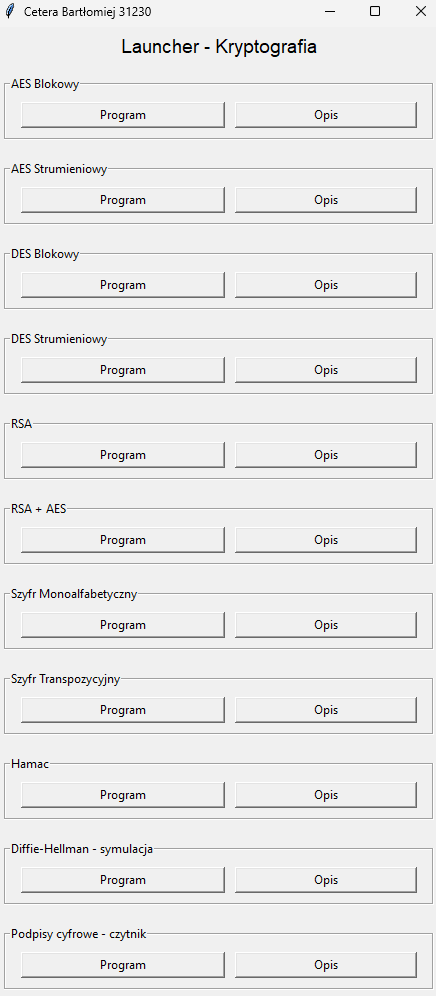
\includegraphics[scale=0.45]{pictures/launcher.png}
\caption{Launcher - aplikacja startowa}
\label{fig:launcher_startowa}
\end{center}
\end{figure}



\subsection{AES}
\subsubsection{AES strumieniowy}
\begin{quotation} \noindent Program AES strumieniowy implementuje algorytm Advanced Encryption Standard (AES) w trybie strumieniowym. W odróżnieniu od trybu blokowego, dane są przetwarzane w sposób ciągły, co pozwala na szyfrowanie i deszyfrowanie danych w mniejszych porcjach. Tryb strumieniowy nie wymaga dzielenia danych na bloki o stałej długości ani stosowania paddingu, dzięki czemu jest bardziej elastyczny i efektywny w przypadku danych o nieokreślonej długości, takich jak strumienie multimediów czy dane przesyłane w czasie rzeczywistym. Program oferuje funkcje szyfrowania i deszyfrowania plików, a także umożliwia wprowadzenie i szyfrowanie tekstu bezpośrednio z interfejsu graficznego. Użytkownik może podać klucz szyfrujący, wybrać plik wejściowy i zapisać zaszyfrowane lub odszyfrowane dane w pliku wynikowym. Klucz musi spełniać wymagania algorytmu AES (128, 192 lub 256 bitów), co gwarantuje bezpieczeństwo operacji.\newline

\noindent\textbf{Scenariusz użycia programu}
\begin{itemize}
\item  Po uruchomieniu programu użytkownik widzi interfejs graficzny, który umożliwia wprowadzenie klucza szyfrującego oraz wybór plików do przetworzenia.
\item Użytkownik podaje klucz szyfrujący w odpowiednim polu tekstowym. Program sprawdza długość klucza, aby upewnić się, że jest zgodna z wymogami AES.
\item Użytkownik może wprowadzić dowolny tekst w polu tekstowym i kliknąć przycisk „Zaszyfruj tekst”, aby zaszyfrować dane i zapisać je do pliku. Szyfrowanie odbywa się strumieniowo, znak po znaku.
\item Użytkownik wybiera plik do zaszyfrowania, wskazuje miejsce zapisu pliku wynikowego, a następnie uruchamia proces szyfrowania. Algorytm AES w trybie strumieniowym szyfruje dane w małych porcjach, dzięki czemu proces jest bardziej elastyczny w przypadku dużych plików.
\item Użytkownik wskazuje plik zaszyfrowany jako wejściowy, wybiera lokalizację dla odszyfrowanego pliku, a następnie uruchamia proces deszyfrowania. 
\item Po zakończeniu szyfrowania lub deszyfrowania użytkownik otrzymuje powiadomienie o sukcesie operacji, a plik wynikowy jest zapisany w wybranej lokalizacji.
\end{itemize}
\end{quotation}

\begin{figure}[!htb]
\begin{center}
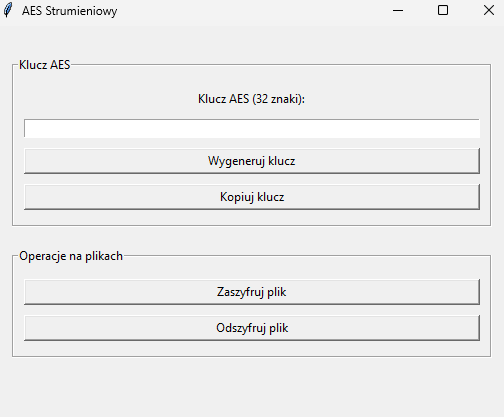
\includegraphics[scale=0.45]{pictures/aesstrumieniowy.png}
\caption{AES strumieniowy}
\label{fig:AES strumieniowy}
\end{center}
\end{figure}

\newpage
\subsubsection{AES blokowy}
\begin{quotation} \noindent Program AES blokowy implementuje algorytm Advanced Encryption Standard (AES) w trybie blokowym. Oznacza to, że dane wejściowe są dzielone na bloki o stałej długości (zazwyczaj 128 bitów), które są szyfrowane indywidualnie, blok po bloku. W przypadku, gdy dane wejściowe nie są wielokrotnością długości bloku, stosowany jest padding, czyli uzupełnianie brakujących bitów. Tryb blokowy oznacza, że każda porcja danych jest przetwarzana w wyraźnie odseparowanych jednostkach (blokach), co różni się od trybu strumieniowego, w którym dane są przetwarzane w sposób ciągły. Program oferuje funkcje zarówno szyfrowania, jak i deszyfrowania plików. Jego graficzny interfejs użytkownika (GUI) umożliwia użytkownikowi wprowadzenie klucza szyfrującego, wybranie pliku wejściowego oraz wskazanie miejsca zapisu wyniku szyfrowania lub deszyfrowania. Klucz wykorzystywany w algorytmie AES musi mieć określoną długość (128, 192 lub 256 bitów), co zapewnia bezpieczeństwo operacji.\newline

\noindent\textbf{Scenariusz użycia programu}
\begin{itemize}
\item Uruchomienie programu: Po uruchomieniu programu użytkownik widzi interfejs graficzny z polami do wprowadzenia klucza szyfrującego oraz przyciskami umożliwiającymi wybór plików do zaszyfrowania lub odszyfrowania.
\item Wprowadzenie klucza: Użytkownik wpisuje w odpowiednie pole klucz szyfrujący. Program automatycznie sprawdza poprawność długości klucza, aby spełniał wymagania algorytmu AES.
\item Wybór pliku do zaszyfrowania: Użytkownik wybiera plik wejściowy, który ma zostać zaszyfrowany, korzystając z przycisku „Wybierz plik”. Następnie wskazuje miejsce, w którym zaszyfrowany plik ma zostać zapisany.
\item Proces szyfrowania: Po kliknięciu przycisku „Szyfruj” program wykorzystuje algorytm AES w trybie blokowym, dzieląc dane na bloki i szyfrując je indywidualnie. Wynik operacji jest zapisywany w pliku wyjściowym.
\item Odszyfrowanie pliku: Aby odszyfrować wcześniej zaszyfrowany plik, użytkownik wskazuje zaszyfrowany plik jako wejściowy oraz wybiera miejsce zapisu odszyfrowanych danych. Po kliknięciu przycisku „Deszyfruj” program odtwarza oryginalne dane z zaszyfrowanych bloków przy użyciu tego samego klucza szyfrującego.
\item Wynik operacji: Po zakończeniu szyfrowania lub deszyfrowania użytkownik otrzymuje komunikat o sukcesie operacji, a plik wynikowy jest zapisany w określonej lokalizacji.
\end{itemize}
\end{quotation}

\begin{figure}[!htb]
\begin{center}
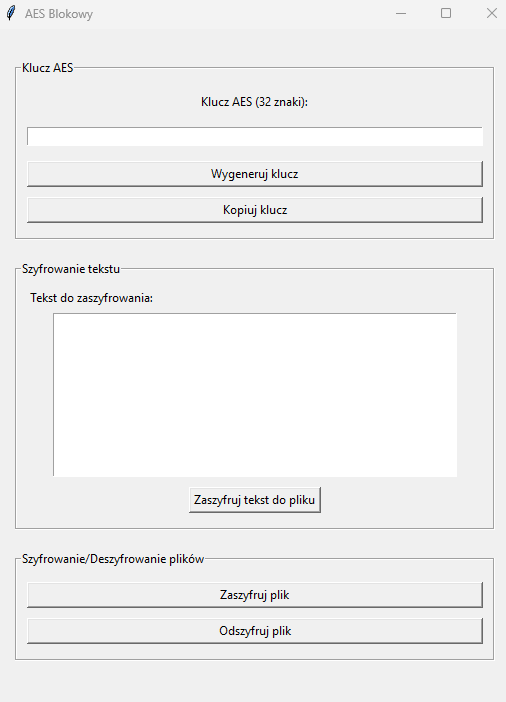
\includegraphics[scale=0.45]{pictures/aesblokowy.png}
\caption{AES blokowy}
\label{fig:AES blokowy}
\end{center}
\end{figure}

\newpage
\subsection{DES}
\subsubsection{DES strumieniowy}
\begin{quotation} \noindent Program DES strumieniowy implementuje algorytm szyfrowania Data Encryption Standard (DES) w trybie strumieniowym. DES, choć historycznie uznawany za standard kryptografii symetrycznej, w swojej strumieniowej wersji pozwala na przetwarzanie danych w mniejszych porcjach, co zwiększa jego elastyczność w przypadku danych o dynamicznej długości lub przesyłanych w czasie rzeczywistym. Tryb strumieniowy nie wymaga dzielenia danych na bloki o stałej długości, co pozwala na szyfrowanie strumieniowe w sposób bardziej zbliżony do rzeczywistych potrzeb użytkownika. Program oferuje użytkownikowi możliwości szyfrowania i deszyfrowania danych, zarówno w postaci plików, jak i tekstu wprowadzanego bezpośrednio w interfejsie. Klucz szyfrujący jest podawany przez użytkownika, co pozwala na pełną kontrolę nad procesem kryptograficznym.\newline

\noindent\textbf{Scenariusz użycia programu}
\begin{itemize}
\item Uruchomienie programu: Po uruchomieniu użytkownik widzi intuicyjny interfejs graficzny, umożliwiający wprowadzenie klucza szyfrującego i wybór operacji szyfrowania lub deszyfrowania.
\item Wprowadzenie klucza: Użytkownik podaje klucz szyfrujący w odpowiednim polu tekstowym. Klucz musi spełniać wymogi DES, czyli być 56-bitowy (często wprowadzany w formie 8 bajtów, z których każdy ma ustawiony 1 bit parzystości).
\item Szyfrowanie tekstu: Użytkownik wprowadza tekst w oknie tekstowym i klika przycisk „Zaszyfruj tekst”. Program przetwarza dane w trybie strumieniowym, zapisując wynik w wybranym pliku.
\item Szyfrowanie pliku: Użytkownik wybiera plik do zaszyfrowania oraz lokalizację zapisu pliku wynikowego. Algorytm DES w trybie strumieniowym przetwarza plik porcjami, co umożliwia szyfrowanie nawet dużych danych bez konieczności ich pełnego wczytania do pamięci.
\item Deszyfrowanie pliku: W procesie deszyfrowania użytkownik wybiera zaszyfrowany plik wejściowy i wskazuje lokalizację pliku wynikowego. Program odtwarza oryginalne dane przy użyciu podanego klucza.
\item Zakończenie operacji: Po zakończeniu procesu szyfrowania lub deszyfrowania użytkownik otrzymuje informację o sukcesie, a plik wynikowy jest dostępny w wybranej lokalizacji.
\end{itemize}
\end{quotation}

\begin{figure}[!htb]
\begin{center}
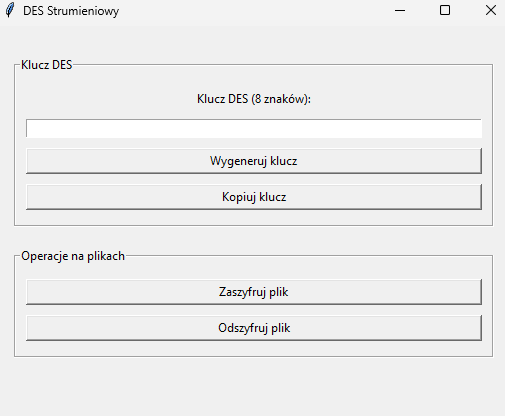
\includegraphics[scale=0.45]{pictures/desstrumieniowy.png}
\caption{DES strumieniowy}
\label{fig:DES strumieniowy}
\end{center}
\end{figure}


\newpage
\subsubsection{DES blokowy}
\begin{quotation} 
\noindent Program DES blokowy implementuje algorytm szyfrowania Data Encryption Standard (DES) w trybie blokowym. DES, jako kryptograficzny algorytm symetryczny, działa na danych w stałych blokach o długości 64 bitów, co odróżnia go od trybu strumieniowego. W trybie blokowym dane wejściowe są dzielone na bloki o ustalonej długości, a każdy z bloków jest przetwarzany niezależnie. Jeśli dane wejściowe nie są wielokrotnością długości bloku, dodawany jest padding, aby wypełnić brakujące bity. Program umożliwia szyfrowanie i deszyfrowanie zarówno tekstu, jak i plików. Użytkownik ma możliwość pracy z kluczem szyfrującym, który musi być zgodny z wymogami DES, a operacje są łatwo dostępne dzięki przyjaznemu interfejsowi graficznemu.\newline

\noindent\textbf{Scenariusz użycia programu}
\begin{itemize}
\item Uruchomienie programu: Użytkownik uruchamia program i wita go interfejs graficzny z opcjami generowania klucza, szyfrowania i deszyfrowania.
\item Generowanie lub wprowadzenie klucza: Użytkownik może wygenerować klucz szyfrujący lub wprowadzić własny klucz. Klucz musi spełniać wymogi algorytmu DES (zazwyczaj 56-bitowy klucz z dodatkowym bitem parzystości).
\item Szyfrowanie tekstu: Użytkownik wprowadza tekst do pola tekstowego i klika przycisk „Zaszyfruj tekst”. Program dzieli tekst na bloki, szyfruje każdy blok i zapisuje wynik w pliku wyjściowym.
\item Szyfrowanie pliku: Użytkownik wybiera plik wejściowy i podaje lokalizację pliku wynikowego. Program dzieli plik na bloki 64-bitowe, dodaje padding (jeśli to konieczne), a następnie szyfruje dane blok po bloku.
\item Deszyfrowanie pliku: Podczas deszyfrowania użytkownik wybiera zaszyfrowany plik i podaje lokalizację pliku wynikowego. Program odtwarza oryginalne dane poprzez usuwanie paddingu i odwrócenie procesu szyfrowania.
\item Informacja o zakończeniu operacji: Po każdej operacji program informuje użytkownika o sukcesie, a dane wynikowe są dostępne w wybranej lokalizacji.
\end{itemize}
\end{quotation}

\begin{figure}[!htb]
\begin{center}
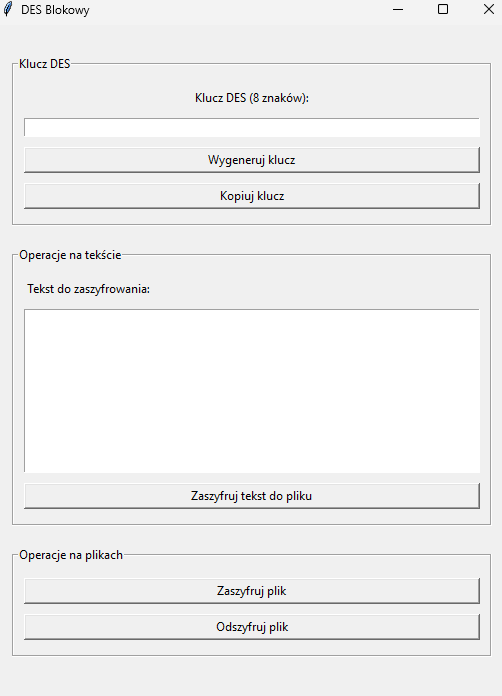
\includegraphics[scale=0.45]{pictures/desblokowy.png}
\caption{DES blokowy}
\label{fig:DES blokowy}
\end{center}
\end{figure}


\newpage
\subsection{RSA}
\begin{quotation} \noindent Program RSA implementuje klasyczny algorytm szyfrowania i deszyfrowania oparty na RSA (Rivest-Shamir-Adleman). RSA to asymetryczny algorytm kryptograficzny, który korzysta z dwóch różnych kluczy: publicznego do szyfrowania oraz prywatnego do deszyfrowania. Program umożliwia generowanie kluczy w sposób prosty i intuicyjny, co stanowi podstawę późniejszych operacji na danych. Główne funkcje programu obejmują szyfrowanie i deszyfrowanie zarówno tekstu, jak i plików. Użytkownik może wprowadzać tekst w dedykowanym polu interfejsu graficznego, który następnie zostaje zaszyfrowany za pomocą klucza publicznego i zapisany w pliku. W przypadku plików program dzieli je na fragmenty zgodne z rozmiarem klucza, co pozwala na ich poprawne szyfrowanie i późniejsze deszyfrowanie.\newline

\noindent\textbf{Scenariusz użycia programu}
\begin{itemize}
\item Użytkownik uruchamia program i generuje parę kluczy (publiczny i prywatny) za pomocą przycisku w interfejsie.
\item Następnie wprowadza tekst do szyfrowania w odpowiednim polu lub wybiera plik do zaszyfrowania.
\item Program szyfruje tekst/plik za pomocą klucza publicznego i zapisuje wynik w wybranej lokalizacji.
\item W przypadku deszyfrowania użytkownik wybiera zaszyfrowany plik i podaje klucz prywatny. Program odszyfrowuje dane i zapisuje wynik w formie odczytywalnej.
\end{itemize}
\end{quotation}

\begin{figure}[!htb]
\begin{center}
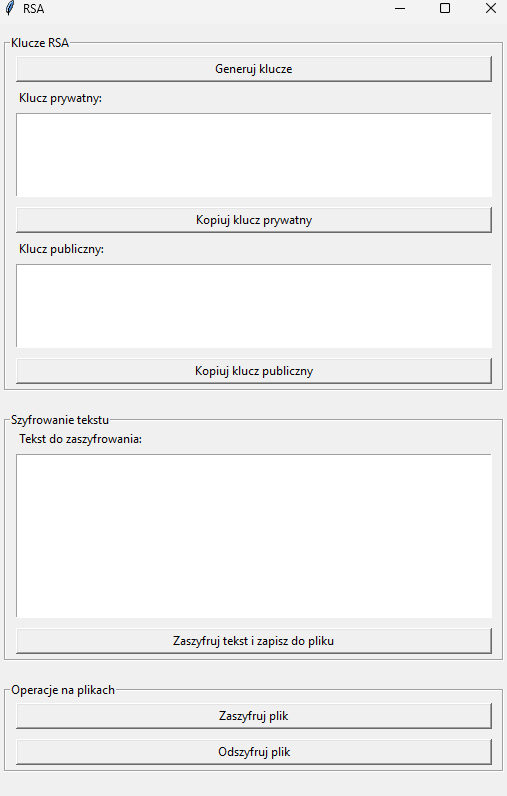
\includegraphics[scale=0.45]{pictures/rsa.png}
\caption{RSA}
\label{fig:RSA}
\end{center}
\end{figure}


\newpage
\subsubsection{RSA + AES}
\begin{quotation} \noindent Program RSA + AES, znajdujący się w podfolderze "RSA" w projekcie, implementuje hybrydowy system kryptograficzny, który łączy zalety asymetrycznego RSA i symetrycznego AES. Tego rodzaju podejście umożliwia efektywne szyfrowanie dużych plików, zachowując jednocześnie wysoki poziom bezpieczeństwa kluczy dzięki kryptografii asymetrycznej. Główne funkcje programu obejmują generowanie par kluczy RSA (prywatnego i publicznego), szyfrowanie tekstu oraz szyfrowanie i deszyfrowanie plików. W przypadku szyfrowania plików stosowany jest schemat hybrydowy: klucz symetryczny AES jest generowany dynamicznie i szyfrowany kluczem publicznym RSA, natomiast rzeczywiste dane pliku są szyfrowane algorytmem AES w trybie EAX, który zapewnia zarówno poufność, jak i integralność danych.\newline

\noindent\textbf{Scenariusz użycia programu}
\begin{itemize}
\item Generowanie kluczy: Użytkownik otwiera aplikację i klika przycisk "Generuj klucze". Program tworzy parę kluczy RSA (prywatny i publiczny). Klucze są wyświetlane w polach tekstowych w interfejsie i mogą być zapisane, skopiowane do schowka lub wykorzystane od razu.
\item Szyfrowanie tekstu: W polu tekstowym użytkownik wpisuje wiadomość, np. "Poufne dane dotyczące projektu". Następnie klika przycisk "Zaszyfruj tekst i zapisz do pliku". Program szyfruje wiadomość przy użyciu klucza publicznego RSA i zapisuje wynik w wybranym przez użytkownika pliku.
\item Szyfrowanie pliku: Użytkownik wskazuje plik do zaszyfrowania, np. dokument "dokumentprojektu.pdf". Program generuje klucz AES i szyfruje plik przy jego użyciu. Klucz AES jest następnie zaszyfrowany kluczem publicznym RSA i zapisany razem z zaszyfrowanym plikiem. Plik wynikowy jest zapisany w wybranej lokalizacji.
\item Przesyłanie zaszyfrowanych danych: Zaszyfrowany plik i klucz publiczny są przesyłane do innego użytkownika, który ma dostęp do klucza prywatnego RSA.
\item Deszyfrowanie pliku: Odbiorca otwiera aplikację, wczytuje swój klucz prywatny RSA i wskazuje zaszyfrowany plik. Program odszyfrowuje klucz AES za pomocą klucza prywatnego RSA, a następnie deszyfruje właściwy plik przy użyciu tego klucza AES. Wynikowy plik jest zapisany w wybranej przez odbiorcę lokalizacji.
\item Weryfikacja: Odbiorca otwiera odszyfrowany plik, który jest identyczny z oryginalnym dokumentem przesłanym przez nadawcę.
\end{itemize}
\end{quotation}

\begin{figure}[!htb]
\begin{center}
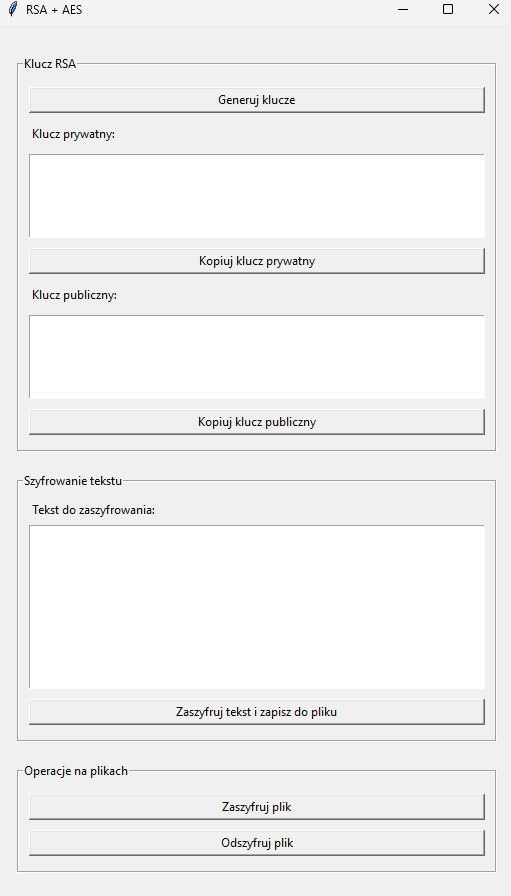
\includegraphics[scale=0.45]{pictures/rsaaes.png}
\caption{RSA + AES}
\label{fig:RSA + AES}
\end{center}
\end{figure}

\newpage
\subsection{Szyfr Monoalfabetyczny}
\begin{quotation} \noindent Program Szyfr Monoalfabetyczny implementuje szyfrowanie i deszyfrowanie tekstu za pomocą szyfru monoalfabetycznego. Szyfr ten polega na podstawieniu każdej litery alfabetu za pomocą odpowiedniego klucza w postaci permutacji liter. Dzięki swojej prostocie jest jednym z najstarszych i najbardziej znanych sposobów szyfrowania, jednak z powodu ograniczonego bezpieczeństwa znajduje obecnie zastosowanie głównie w celach edukacyjnych. Program umożliwia użytkownikowi szyfrowanie tekstu poprzez wpisanie go w odpowiednie pole w interfejsie, a następnie przekształca go zgodnie z określonym kluczem szyfrującym i zapisuje wynik w pliku. W podobny sposób można odszyfrować tekst, który został wcześniej zaszyfrowany przy użyciu tego samego klucza, co pozwala na odzyskanie pierwotnej zawartości. Program obsługuje również szyfrowanie i deszyfrowanie plików tekstowych, oferując użytkownikowi możliwość wskazania pliku do przetworzenia oraz miejsca zapisu wyniku. Dzięki intuicyjnemu interfejsowi aplikacja jest przystępna w użyciu i wspiera naukę podstawowych zasad działania prostych algorytmów szyfrowania.\newline

\noindent\textbf{Scenariusz użycia programu}
\begin{itemize}
\item Użytkownik otwiera aplikację i generuje klucz szyfrujący, który jest permutacją alfabetu (np. qwertyuiopasdfghjklzxcvbnm).
\item Użytkownik wpisuje tekst w pole, np. "To jest test", a następnie wybiera opcję zaszyfrowania. Program używa klucza do zamiany każdej litery tekstu na odpowiadającą literę z permutacji i zapisuje wynik w pliku.
\item Zaszyfrowany tekst, np. "Yg oyjg ygst", może zostać przesłany do innej osoby, która posiada odpowiedni klucz odszyfrowujący.
\item Odbiorca wprowadza zaszyfrowany tekst do programu, używa tego samego klucza i odtwarza pierwotny tekst.
\end{itemize}
\end{quotation}

\begin{figure}[!htb]
\begin{center}
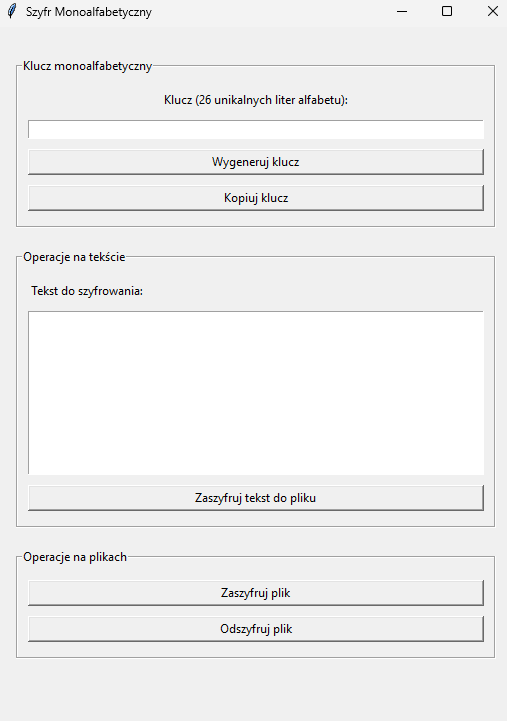
\includegraphics[scale=0.45]{pictures/monoalfabetyczny.png}
\caption{Szyfr Monoalfabetyczny}
\label{fig:Szyfr Monoalfabetyczny}
\end{center}
\end{figure}


\newpage
\subsection{Szyfr Transpozycyjny}
\begin{quotation} \noindent Program Szyfr Transpozycyjny implementuje algorytm szyfrowania i deszyfrowania oparty na zasadzie przestawiania (transpozycji) znaków w tekście. W szyfrze transpozycyjnym kolejność liter w tekście jest zmieniana według określonego schematu, który opiera się na kluczu wskazującym, w jaki sposób należy przestawić znaki. W przeciwieństwie do szyfrów podstawieniowych, takich jak monoalfabetyczny, szyfr transpozycyjny nie zmienia wartości znaków, a jedynie ich kolejność, co zapewnia inny rodzaj ukrywania informacji. Program umożliwia użytkownikowi szyfrowanie tekstu poprzez wpisanie go w dedykowane pole w interfejsie. Na podstawie wprowadzonego klucza (określającego sposób przestawiania znaków) aplikacja generuje tekst zaszyfrowany, który można zapisać do pliku. W analogiczny sposób użytkownik może odszyfrować tekst, przywracając jego pierwotną kolejność znaków, o ile użyje tego samego klucza, który został zastosowany podczas szyfrowania. Program obsługuje także szyfrowanie i deszyfrowanie plików tekstowych, co pozwala na wygodne przetwarzanie większych zbiorów danych.\newline

\noindent\textbf{Scenariusz użycia programu}
\begin{itemize}
\item Użytkownik uruchamia aplikację i widzi interfejs z polami do wprowadzania tekstu, wybierania plików oraz klucza szyfrującego.
\item Wprowadza tekst, który chce zaszyfrować, np. "Witaj świecie", i podaje klucz, np. 4.
\item Po kliknięciu przycisku "Szyfruj tekst i zapisz do pliku" program przetwarza tekst, tworząc zaszyfrowaną wersję, i zapisuje ją w wybranym pliku.
\item Aby odszyfrować tekst, użytkownik wskazuje zaszyfrowany plik i ponownie wprowadza ten sam klucz. Po kliknięciu "Odszyfruj plik" program odtwarza pierwotny tekst i zapisuje go w nowym pliku.
\item Użytkownik może również szyfrować lub odszyfrowywać całe pliki tekstowe, wybierając je w odpowiednich sekcjach aplikacji.
\end{itemize}
\end{quotation}

\begin{figure}[!htb]
\begin{center}
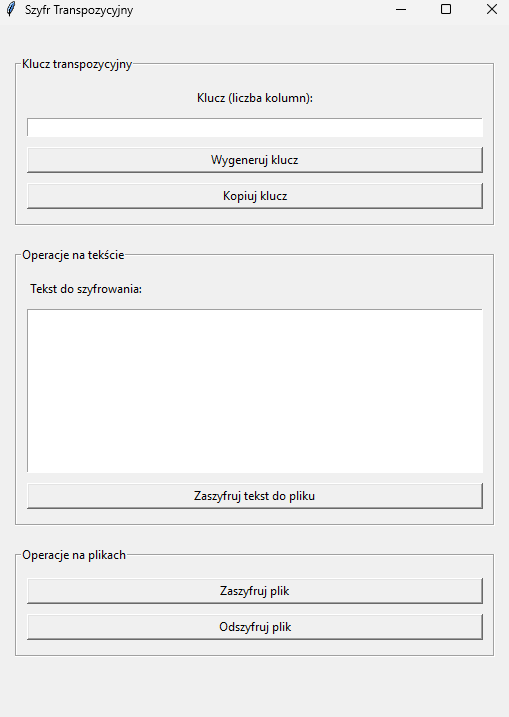
\includegraphics[scale=0.45]{pictures/transpozycyjny.png}
\caption{Szyfr Transpozycyjny}
\label{fig:Szyfr Transpozycyjny}
\end{center}
\end{figure}


\newpage
\subsection{HAMAC}
\begin{quotation} \noindent Program HMAC (Hash-based Message Authentication Code) realizuje funkcjonalność opartą na algorytmie kryptograficznym, który umożliwia uwierzytelnianie wiadomości i weryfikację ich integralności. Wykorzystuje funkcję skrótu, taką jak SHA-256, oraz klucz kryptograficzny do generowania kodu uwierzytelniającego (HMAC), który jest unikalny dla danej wiadomości i klucza. Program pozwala na generowanie jednego klucza kryptograficznego, który jest wykorzystywany zarówno do generowania kodów HMAC, jak i do ich weryfikacji, a klucz ten może być zapisywany i kopiowany. Użytkownik może wpisać wiadomość w polu tekstowym i za pomocą przycisku utworzyć jej kod HMAC, który zostanie zapisany do pliku. Program umożliwia także wybranie pliku, dla którego wygenerowany zostanie kod HMAC, a wynikowa wartość zapisana w wybranym pliku wyjściowym. Wygenerowany HMAC można porównać z istniejącą wartością, aby upewnić się, że dane nie zostały zmienione. Dzięki temu program demonstruje praktyczne zastosowanie generowania i weryfikacji HMAC w prosty i intuicyjny sposób.\newline

\noindent\textbf{Scenariusz użycia programu}
\begin{itemize}
\item Użytkownik uruchamia aplikację i generuje klucz kryptograficzny.
\item Wpisuje tekst do pola w aplikacji, klika przycisk generowania HMAC, a wynik zapisuje do pliku.
\item Następnie użytkownik wybiera plik tekstowy, generuje dla niego kod HMAC i zapisuje wynik w oddzielnym pliku.
\item W późniejszym czasie, przy użyciu tego samego klucza, użytkownik może zweryfikować oryginalność danych, porównując zapisany HMAC z wartością ponownie wygenerowaną dla danego pliku lub wiadomości.
\end{itemize}
\end{quotation}

\begin{figure}[!htb]
\begin{center}
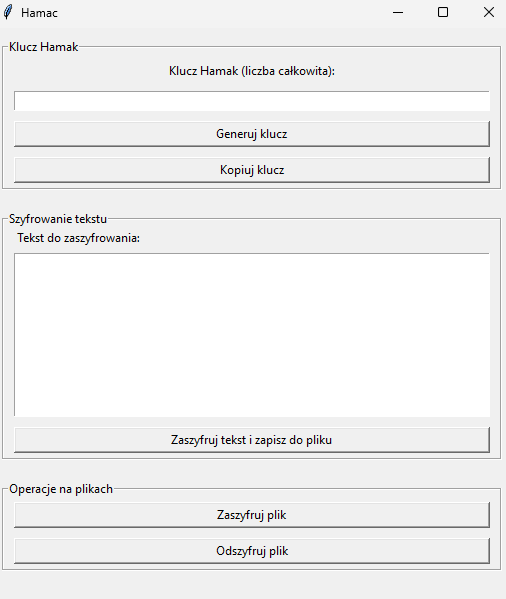
\includegraphics[scale=0.45]{pictures/hamac.png}
\caption{HAMAC}
\label{fig:HAMAC}
\end{center}
\end{figure}


\newpage
\subsection{Diffie-Hellman - symulacja}
\begin{quotation} \noindent Program symulacji protokołu Diffie-Hellmana pozwala użytkownikom zrozumieć, jak działa proces wymiany kluczy w systemie kryptograficznym opartym na trudności rozwiązania problemu logarytmu dyskretnego. Protokół ten umożliwia dwóm stronom obliczenie wspólnego tajnego klucza na podstawie publicznie wymienionych danych, takich jak baza i liczba pierwsza. W programie każda strona, reprezentowana przez Alicję i Boba, generuje swój klucz prywatny oraz odpowiadający mu klucz publiczny. Po wymianie kluczy publicznych obie strony obliczają identyczny wspólny klucz przy użyciu swoich kluczy prywatnych i publicznych drugiej strony.\newline
\end{quotation}

\begin{figure}[!htb]
\begin{center}
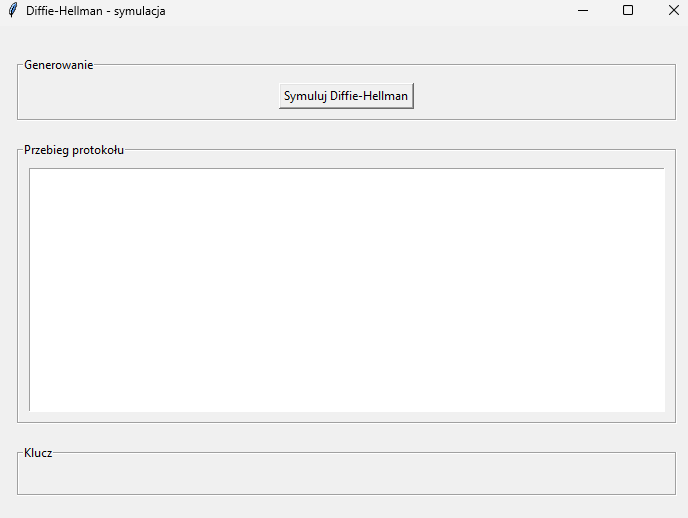
\includegraphics[scale=0.45]{pictures/dfsymulacja.png}
\caption{Diffie-Hellman - symulacja}
\label{fig:Diffie-Hellman - symulacja}
\end{center}
\end{figure}

\subsection{Podpisy cyfrowe - czytnik}
\begin{quotation} \noindent „Podpisy cyfrowe – czytnik” służy do analizy podpisów cyfrowych w plikach PDF. Umożliwia wczytanie dokumentu, a następnie sprawdzenie szczegółów podpisów, takich jak dane podpisującego, powód podpisu, data podpisania oraz informacje o użytych certyfikatach. Dzięki prostemu interfejsowi użytkownik może łatwo wyświetlić i zrozumieć strukturę podpisów cyfrowych. Aplikacja analizuje zawartość podpisu i prezentuje informacje w czytelnej formie, co pozwala na weryfikację, czy dokument został prawidłowo podpisany i czy nie uległ zmianom. Narzędzie sprawdza się zarówno dla osób uczących się o podpisach cyfrowych, jak i dla profesjonalistów, którzy potrzebują szybko zweryfikować autentyczność podpisanych dokumentów.\newline
\end{quotation}

\begin{figure}[!htb]
\begin{center}
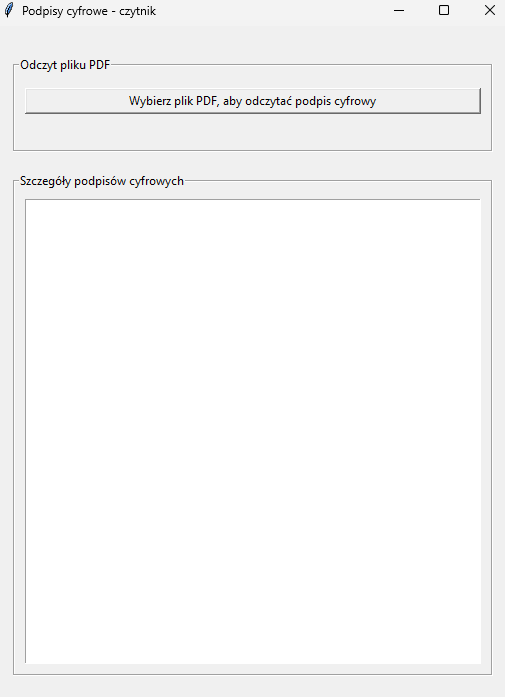
\includegraphics[scale=0.45]{pictures/podpisy.png}
\caption{Podpisy cyfrowe - czytnik}
\label{fig:Podpisy cyfrowe - czytnik}
\end{center}
\end{figure}

\subsection{Kod Huffmana}
\begin{quotation} \noindent Program wykorzystuje on algorytm kodowania Huffmana, który przypisuje zmiennobitowe kody binarne symbolom w zależności od ich częstotliwości występowania. Algorytm działa w oparciu o drzewo Huffmana, w którym symbole o wyższej częstotliwości są reprezentowane przez krótsze kody, co pozwala efektywnie zmniejszyć rozmiar danych bez utraty informacji. Program umożliwia użytkownikowi zarówno szyfrowanie tekstu i plików, jak i ich późniejsze odszyfrowanie. Działanie programu opiera się na trzech głównych modułach: szyfrowania, deszyfrowania oraz interfejsu graficznego. Moduł szyfrowania odczytuje dane wejściowe (tekst lub zawartość pliku), analizuje częstotliwość występowania symboli i buduje drzewo Huffmana. Na podstawie drzewa generowane są kody binarne przypisywane każdemu symbolowi, które następnie są używane do zakodowania danych. Wynikowe dane zakodowane, wraz z informacją o strukturze drzewa Huffmana, są zapisywane do pliku w formacie binarnym. Moduł deszyfrowania wykorzystuje zapisane drzewo Huffmana do interpretacji zakodowanych danych. Po odczytaniu bitów użytkownik odtwarza oryginalne dane, poruszając się po drzewie Huffmana od korzenia do liści, zgodnie z odczytanymi bitami (0 dla lewej gałęzi, 1 dla prawej). Program gwarantuje, że wynik deszyfrowania będzie identyczny z pierwotnymi danymi wejściowymi, pod warunkiem, że nie nastąpiła ich modyfikacja w czasie przesyłu.\newline

\noindent\textbf{Scenariusz użycia programu}
\begin{itemize}
\item Użytkownik uruchamia aplikację i wprowadza tekst w polu tekstowym.
\item Klika przycisk „Zaszyfruj tekst do pliku”, aby zapisać zaszyfrowaną wersję tekstu w formacie Huffmana.
\item Użytkownik wybiera plik do zaszyfrowania, klikając przycisk „Zaszyfruj plik”. Plik jest przetwarzany, a jego zakodowana wersja zapisywana do pliku wyjściowego.
\item W przypadku odszyfrowania użytkownik wybiera zaszyfrowany plik Huffmana i klika „Odszyfruj plik”. Program odtwarza oryginalne dane, zapisując je w wybranym pliku wyjściowym.
\item Wyniki operacji (np. sukces, błędy) są wyświetlane w komunikatach okienkowych, co umożliwia łatwą kontrolę działania programu.
\end{itemize}
\end{quotation}

\begin{figure}[!htb]
\begin{center}
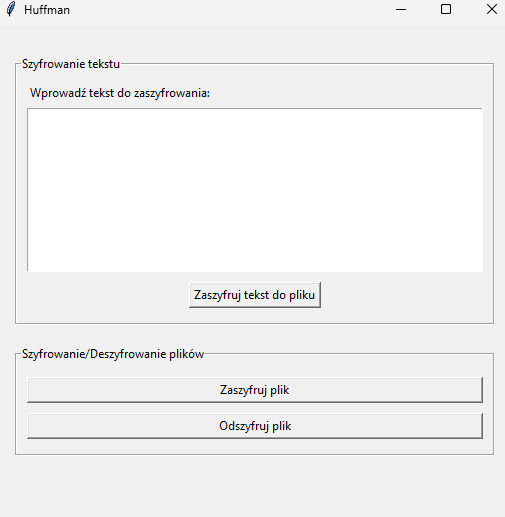
\includegraphics[scale=0.45]{pictures/huffman.png}
\caption{Kod Huffmana}
\label{fig:Kod Huffmana}
\end{center}
\end{figure}

\subsection{Symulacja Kodowania Hamminga}
\begin{quotation} \noindent Program symulujący działanie kodu Hamminga (7,4) został zaprojektowany, aby wizualizować procesy związane z wykrywaniem i korekcją błędów w danych binarnych. Kod Hamminga umożliwia zarówno wykrycie, jak i poprawienie jednego błędu w przesyłanych lub przechowywanych danych, co jest kluczowe w zapewnianiu niezawodności w systemach cyfrowych. Program umożliwia użytkownikowi interaktywne obserwowanie, jak oryginalne dane są kodowane, jak błąd zostaje losowo wprowadzony do zakodowanych danych, a następnie jak system identyfikuje i koryguje ten błąd, aby odzyskać pierwotne dane.\newline

\noindent\textbf{Scenariusz użycia programu}
\begin{itemize}
\item Użytkownik uruchamia aplikację i klika przycisk „Symuluj kod Hamminga”.
\item Program generuje losowe dane wejściowe (4 bity) i koduje je w bloku Hamminga (7,4).
\item Program losowo wprowadza jeden błąd w zakodowanych danych.
\item Program identyfikuje pozycję błędu, koryguje go i odtwarza pierwotne dane.
\item Wynik procesu (oryginalne dane, zakodowane dane, dane z błędem, pozycja błędu, poprawione dane) jest wyświetlany w oknie aplikacji.
\item Użytkownik może powtarzać symulację, obserwując nowe dane i wyniki.
\end{itemize}
\end{quotation}

\begin{figure}[!htb]
\begin{center}
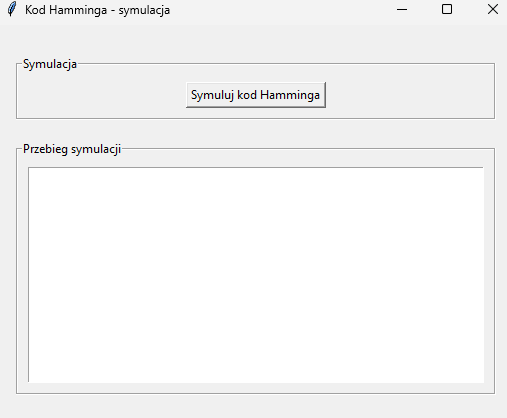
\includegraphics[scale=0.45]{pictures/hamming.png}
\caption{Symulacja Kodowania Hamminga}
\label{fig:Symulacja Kodowania Hamminga}
\end{center}
\end{figure}

\newpage
\section{Podsumowanie}
\noindent Projekt zrealizowany w ramach przedmioty Kryptografia i teoria kodów stanowi kompleksowe narzędzie. Został zaprojektowany w sposób modułowy, co pozwala na łatwe zarządzanie poszczególnymi komponentami oraz ich rozszerzanie. Każdy moduł odpowiada za implementację określonego algorytmu kryptograficznego lub funkcji, takich jak szyfrowanie, deszyfrowanie, generowanie kluczy czy weryfikacja podpisów cyfrowych. Dzięki centralnemu elementowi, jakim jest „launcher”, użytkownicy mają szybki dostęp do wszystkich funkcjonalności aplikacji, co czyni ją intuicyjną i przyjazną dla użytkownika.\newline

\noindent Projekt obejmuje implementację zarówno klasycznych algorytmów, takich jak szyfry monoalfabetyczne i transpozycyjne, jak i zaawansowanych systemów, takich jak AES, DES czy RSA, w tym wersje hybrydowe łączące różne podejścia. Dodatkowo, aplikacja oferuje symulację wymiany kluczy Diffie-Hellmana oraz narzędzie do analizy podpisów cyfrowych, co czyni ją wszechstronnym narzędziem edukacyjnym i użytkowym. Obsługa plików tekstowych i binarnych, wsparcie dla uwierzytelniania wiadomości za pomocą HMAC oraz przyjazny interfejs graficzny umożliwiają wykorzystanie aplikacji w szerokim zakresie scenariuszy.\newline

\noindent Dobór technologii, takich jak Python i jego biblioteki (m.in. PyCryptodome, Tkinter, Pyperclip), pozwolił na połączenie prostoty implementacji z zaawansowaną funkcjonalnością kryptograficzną. Dzięki temu realizacja aplikacji miała istotny wkład w rozwój umiejętności programisty, łącząc teorię z praktyką.


\end{document}